\documentclass{article}[jsarticle]
\usepackage[T1]{fontenc}
\usepackage[dvipdfmx]{hyperref}
\usepackage{lmodern}
\usepackage{latexsym}
\usepackage{amsfonts}
\usepackage{amssymb}
\usepackage{mathtools}
\usepackage{nccmath}
\usepackage{amsthm}
\usepackage{multirow}
\usepackage{graphicx}
\usepackage[dvipdfmx]{color}
\usepackage{wrapfig}
\usepackage{here}
\usepackage{float}
\usepackage{ascmac}
\usepackage{url}
\usepackage{caption}

% Generated by ChatGPT
\usepackage{listings}
\usepackage{xcolor}

\lstset{
    basicstyle=\ttfamily\color{white},
    numbers=none,  % Line numbers
    numberstyle=\tiny\color{white},
    numbersep=5pt,
    tabsize=2,
    extendedchars=true,
    breaklines=true,
    keywordstyle=\color[rgb]{0.58,0.00,0.83},
    stringstyle=\color[rgb]{0.81,0.36,0.00},
    identifierstyle=\color{white},
    commentstyle=\color[rgb]{0.34,0.62,0.16},
    rulecolor=\color[rgb]{0.5,0.5,0.5},
    xleftmargin=0.1cm,    % Left margin
    xrightmargin=0.1cm,   % Right margin
    language=python,
    backgroundcolor=\color[rgb]{0.13,0.13,0.13},
    showspaces=false,
    showstringspaces=false
}



\title{2023年度 研究内容提案書}
\author{高林秀 \\ 三宅研究室 博士前期課程1年 \\ V-CampusID : 23vr008n}
\date{\today}

\begin{document}

\maketitle

\begin{abstract}
    本稿は修士論文執筆に伴う、研究提案を記載するものである.\par
    本稿の構成は,第1章において研究したいテーマとその概要について記載する。第2章において昨年度特別研究1から現在までの研究準備状況を記載する。
    第3章において、修士論文執筆までの研究計画について記載する.\par 
    なお巻末には参考文献と,本稿記載の実験環境を格納したリポジトリのURLを記載する.\par 
    なお、本稿の内容は特別研究2の「研究状況報告書」に記載した内容と同一であるため詳細についてはそちらを参照されたい.
\end{abstract}

\tableofcontents

\section{研究希望テーマ}
本章では修士論文執筆において、希望する研究テーマとその内容、研究背景、研究目標について記載する。

\subsection{研究テーマ}
\centerline{
        \textbf{マルチエージェント強化学習を利用した,} \\
        \textbf{自律型ドローンによる災害対応アプローチ}
    }
    大規模災害時の被災者救助や救援物資輸送の効率化,省人化を目指す.
    具体的には,ドローンとマルチエージェント強化学習(※以下,MARLと呼称)を組み合わせた新たなアプローチを開発し,その有効性を検証する.
\subsection{研究背景}
\paragraph{自衛隊員の不足} \par 
災害大国である我が国において,被災者の捜索,被害状況の把握,
救援物資の現地輸送といった対応は,迅速かつ効率的に行われなければならない.しかし近年,そのような災害対応を一任務とする,
自衛隊員の人材が不足している,あるいは今後さらに不足する事態が予想されている.\par 
以下は\href{http://www.clearing.mod.go.jp/hakusho_data/2022/html/ns056000.html}{令和4年版 防衛白書\cite{doc02}の自衛官の定員及び現員並びに自衛官の定数と現員数の推移に関する資料}である.
\begin{figure}[H]
    \centering
    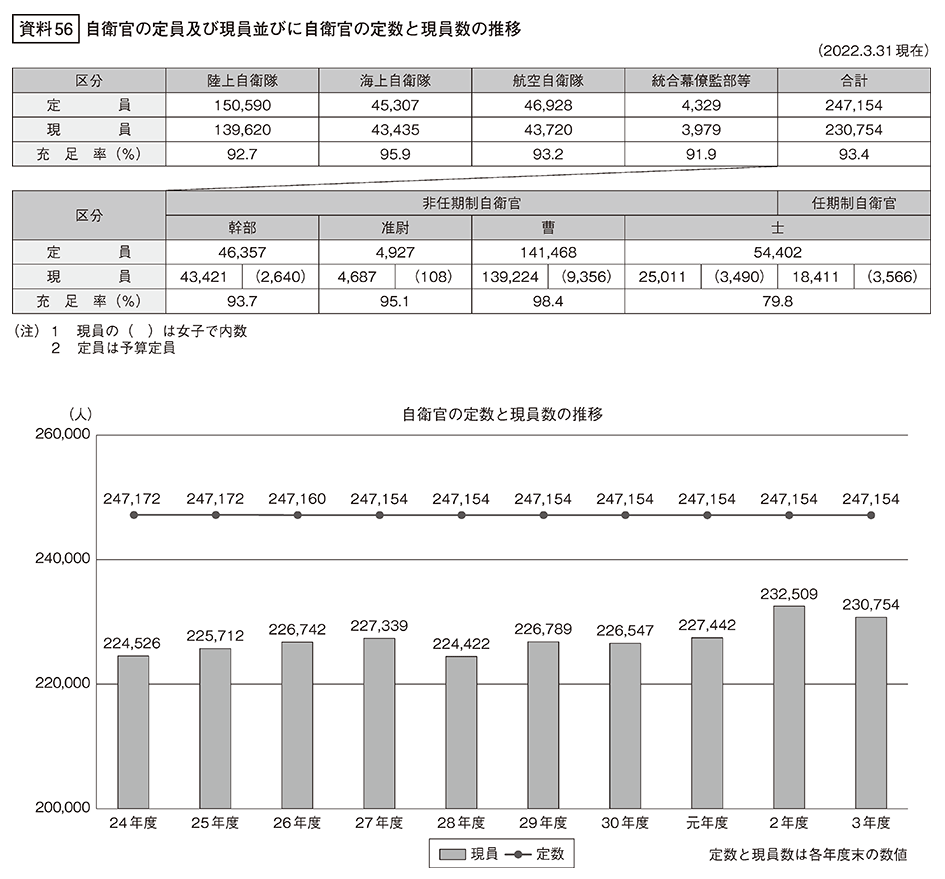
\includegraphics[scale=0.3]{./Images/20240203195052.png}
    \caption{自衛官の定員及び現員並びに自衛官の定数と現員数の推移}
\end{figure}
このように,平成24年度からの統計でも,自衛官の定員数と現員数には$16000$名前後の開きがあり,法律で定められた定員を満たせていない.\par
採用の観点では,2022年度の任期制自衛官の採用で、候補生が計画数の4割ほどしか集まらず、過去最低となった事例がある\cite{news01}.
今後の,少子高齢化が進む我が国において,自衛隊員の不足は深刻な問題となることが予想されている.

\paragraph{陸上自衛隊におけるドローン配備の増強と活用}
防衛省は2020年に,同年末までに陸上自衛隊のドローン配備数を合計201機とすることを発表\cite{news02}していた.
2018年末の時点での配備数は計で13機であったため,大幅な増強をおこなうこととなった.\par
このドローン増強の背景として,2018年9月に発生した北海道胆振東部地震がある.人が入り込めない山奥や広いエリアを短時間で撮影できる利点が評価され,導入が進められた.\par
2019年の防衛白書では,人員の進入困難な箇所や方向から地上部隊がドローンを飛ばし,救助を待つ人がどこにいるかなどの情報を迅速に提供したと明記され,陸上自衛隊の各基地にドローンを1,2機ずつ配備する体制が進んでいた.\par
また,同年2月には,陸上自衛隊東部方面総監部とJUIDA(日本UAS産業振興協議会)\footnote{一般社団法人日本UAS産業振興協議会 JUIDA:我が国における無人航空機
の産業振興を目的に2014年7月に設立された.無人航空機の情報周知活動や,航行ガイドラインの策定,市場創造支援などに取り組んでいる.}が大規模災害発生時における相互協力を目的とした協定を締結しており,今後自衛隊の災害派遣においてドローンの利活用がさらに進むことが予想される.
\paragraph{レベル4飛行の解禁} \par
レベル4飛行とは,有人地帯での目視外飛行のこと.目視で監視できない状態で,有人地帯上空を自律飛行することができる飛行レベルを指す.
我が国では2022年12月5日に改正航空法が施行され,レベル4飛行が解禁された\cite{doc01}.\par 
これにより,現在ドローンの災害対応における有効性に注目が集まっている.

\subsection{本研究の新規性}
本研究の新規性について、以下の点を挙げることができる。
\begin{itemize}
    \item 複数機が連携した運用 かつ AIとMARLによるアプローチ
    \item MARLにより他のドローンと連携し、複雑な災害環境下での意思決定を最適化を試みる
    \item 既存の実証事例では、単一のドローンによる物資輸送の事例が多い。
\end{itemize}

\subsection{本研究の目的}
本研究は、災害現場における被害状況偵察や、救急物資の輸送など災害対応におけるドローンの有効性を高めることを目的とする。
また、AIの導入による災害現場での省人化を目的とし、今後少子高齢化が進む我が国における災害対応の新たなアプローチの模索、提案を行うものとする。
\subsection{本研究の到達目標}
本研究は、工学的な応用研究として行うものとする。なお、目指す到達目標は以下の通りである。
\begin{itemize}
    \item MARLとドローンの災害対応への応用可能性の立証。
    \item MARLを導入することによるドローンの連携運用の効果を示す。
    \item 実機での運用を想定したプロトタイプの制作により、運用可能性を示す。
\end{itemize}

\section{研究準備状況}
本章では、2024年2月25日現在における、研究の準備状況について記載する。
昨年度の特別研究1,2における主な取り組みの記載、本年度特別研究3,4を実施するにあたっての課題状況を記載する。
\subsection{昨年度特別研究1,2の取り組み}
昨年度の特別研究1,2では、以下の取り組みを行った。
\begin{itemize}
    \item 過去の大規模災害時の事例調査
    \item 国内における災害時ドローン運用の現状
    \begin{itemize}
        \item ドローンの法整備関する調査
        \item 官公庁の災害時ドローンの運用計画の調査
        \item 国内における運用事例の調査
    \end{itemize}
    \item 関連技術の習得とドローンシミュレーションの構築
    \begin{itemize}
        \item Unity/C\#, ML-Agentsの基礎学習
        \item 飛行制御タスクと、物資空輸タスクの実験
        \item 実機と強化学習モデルの連携に関する技術調査
    \end{itemize}
\end{itemize}
\begin{figure}[H]
    \centering
    \begin{minipage}{0.45\textwidth}
      \centering
      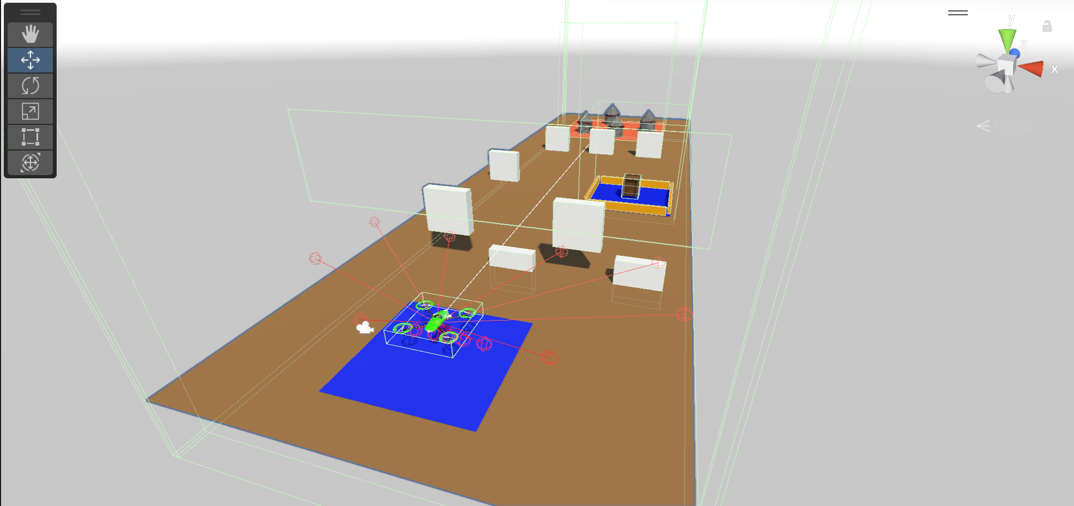
\includegraphics[width=\textwidth]{./Images/202402032208.png} 
      \caption{単一なフィールド内における物資輸送タスクの訓練}
      \label{fig:image1}
    \end{minipage}
    \hfill 
    \begin{minipage}{0.45\textwidth}
      \centering
      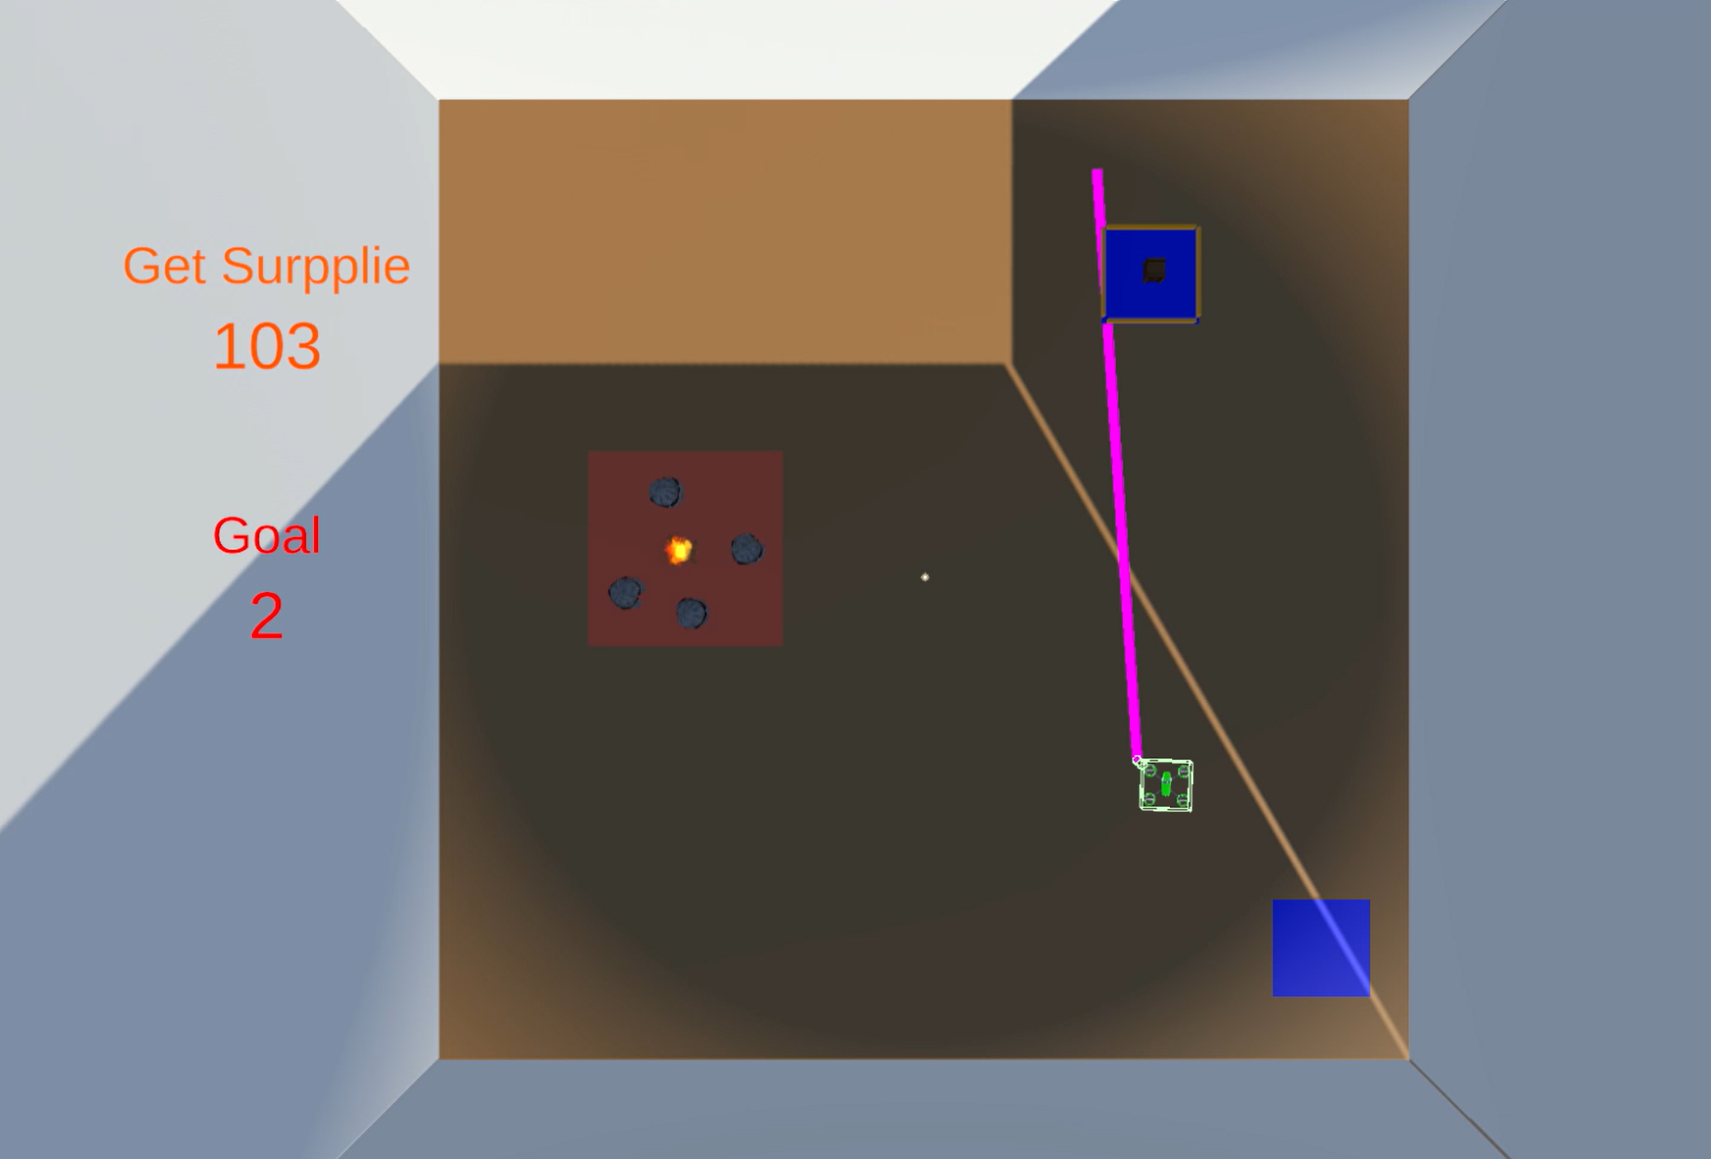
\includegraphics[width=\textwidth]{./Images/20240203221239.png}
      \caption{ナビゲーションAIによる誘導を取り入れ、より効率的に学習できるように改良}
      \label{fig:image2}
    \end{minipage}
  \end{figure}
\subsection{本年度特別研究3,4への課題}
以上の研究準備活動により、今後研究を進める上で、以下の課題が浮き彫りになった。
\begin{itemize}
    \item シミュレーションの問題設定と本研究が対象とする問題設定の具体化
    \begin{itemize}
        \item 災害対応において、MARLが有効な問題の絞り込みが必要
    \end{itemize}
    \item MARLの導入によるドローンの連携運用の効果の客観的な検証方法
    \begin{itemize}
        \item どの様な評価基準を持って、本研究が提案するアプローチの有効性を示すか
    \end{itemize}
\end{itemize}

\section{特別研究3の研究計画}
本章では、2023年2月現在から本年度特別研究3における研究計画について記載する。
\paragraph{2024年 2月~3月}
\begin{itemize}
    \item マルチエージェントでの簡単な物資輸送タスクのシミュレーション開発
    \item マルチエージェント強化学習が災害対応において有効なタスクの調査
    \item 問題設定とシミュレーション内容の具体化
\end{itemize}
\paragraph{2024年 4月~5月}
\begin{itemize}
    \item モデル開発用シミュレーションの開発
    \item モデルの開発
    \item 実機ドローンのプログラム制御飛行試験
    \begin{itemize}
        \item 強化学習モデルとの連携に関連する課題の洗い出し
        \item 解決のための技術調査,開発
    \end{itemize}
\end{itemize}
\paragraph{2024年 6月~7月}
\begin{itemize}
    \item 強化学習モデルと実機ドローンの連携開発
    \item 実機ドローンでの飛行試験
    \item データの収集,分析,修論準備
\end{itemize}
\appendix

\section{参考記事・文献}

\begin{thebibliography}{99}
    \bibitem{news01} 宮崎亜巳、Linda Sieg 田巻一彦 田中志保, 焦点:自衛隊に迫る「静かな有事」、少子化で採用難, ロイター通信, 2018年.
    \begin{itemize}
        \item \url{https://jp.reuters.com/article/idUSKCN1LZ19W/}
    \end{itemize}
    \bibitem{news02} 防衛省、自衛隊のドローン配備拡充 今年度末201機体制、災害救助に活用, 日刊工業新聞, 2019年
    \begin{itemize}
        \item \url{https://www.nikkan.co.jp/articles/view/00558763}
    \end{itemize}
    \bibitem{doc01} 航空法等の一部を改正する法律案を閣議決定, 国土交通省, 2021年
    \begin{itemize}
        \item \url{https://www.mlit.go.jp/report/press/kouku01_hh_000110.html}
    \end{itemize}
    \bibitem{doc02} 令和4年版 防衛白書, 防衛省, 2022年
    \begin{itemize}
        \item \url{http://www.clearing.mod.go.jp/hakusho_data/2022/html/ns056000.html}
    \end{itemize}
\end{thebibliography}

\section{開発リポジトリ、特別研究1,2の提出物URL}
\begin{itemize}
    \item 基礎開発用リポジトリ
    \begin{itemize}
        \item 開発における課題や進捗などは随時こちらのリポジトリに掲載・更新している。
        \item \url{https://github.com/tsyu12345/Learning-MasterPJ_BaseTech}
    \end{itemize}
    \item 研究用GoogleDrive
    \begin{itemize}
        \item 調査した文献や、これまでの研究打合せ資料等を格納している。
        \item \url{https://drive.google.com/drive/folders/11IgJxB2wnGv301JxoCcFtRvTL7CAPbpB}
    \end{itemize}
    \item 研究計画書
    \begin{itemize}
        \item 昨年度特別研究1における提出物
        \item \url{https://drive.google.com/file/d/1g-kUgHJaKJOQFNeQN_SwcILrmPwW75ZD/view?usp=drive_link}
    \end{itemize}
    \item 2024年2月現在の研究状況報告書
    \begin{itemize}
        \item 昨年度特別研究2における提出物
        \item \url{https://drive.google.com/file/d/1Xjr7DCOFj7sh-UnN9JI_Y7gjFOvZVeig/view?usp=drive_link}
    \end{itemize}
\end{itemize}
\end{document}
